\subsection{M.PD.4 - Indice Gulpease}
\begin{figure}[H]
    \centering
    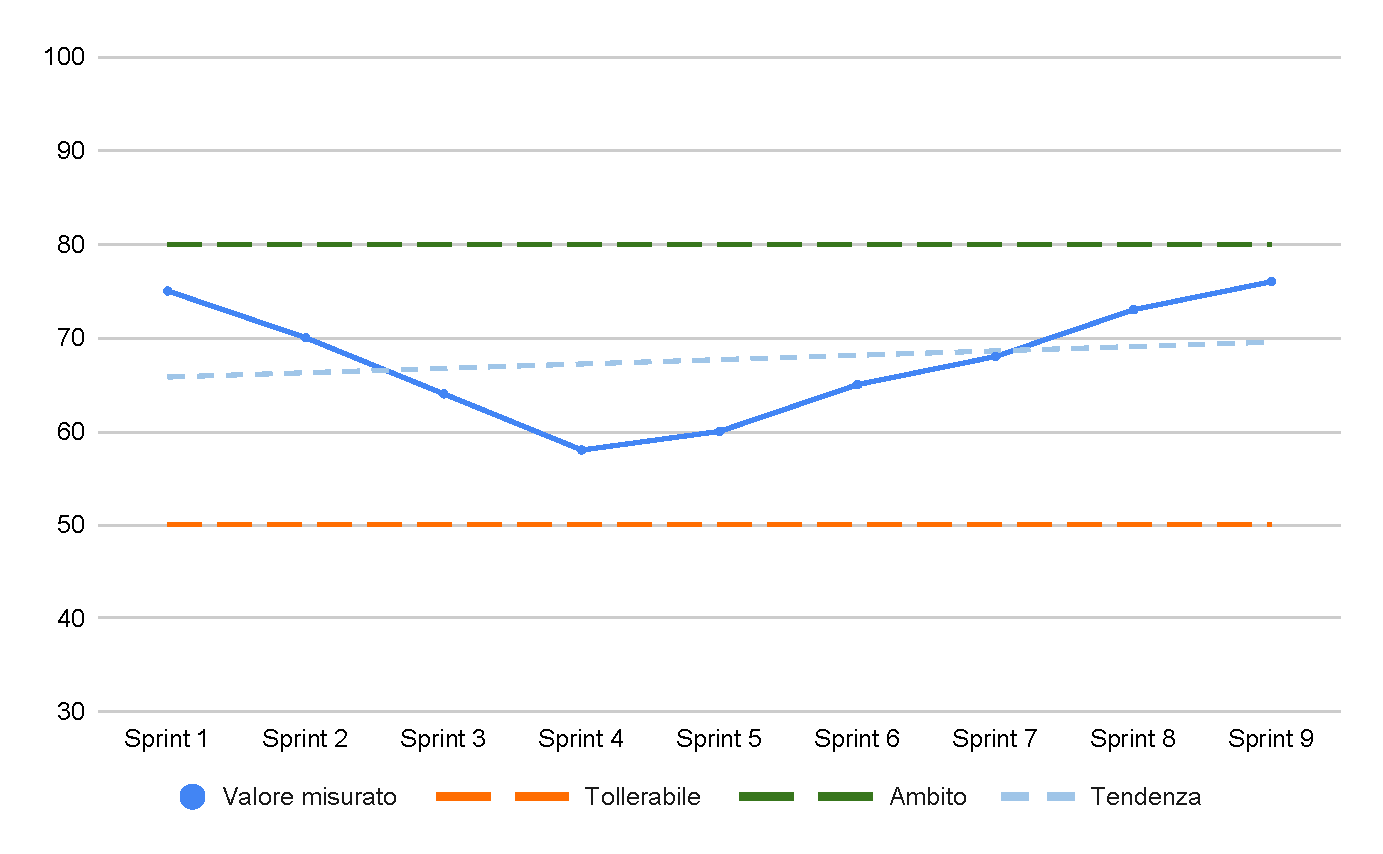
\includegraphics[width=\textwidth]{assets/indice_gulpease.pdf}
    \caption{M.PD.4 - Indice Gulpease}
\end{figure}

\par Il grafico riporta la media degli Indici Gulpease di tutti i documenti, sia interni che esterni. Il valore medio oscilla tra 55 e 78; ciò significa che i documenti sono comprensibili anche per chi possiede una licenza media. I valori più bassi sono stati rilevati nella fase centrale della \glossario{RTB}, poiché il team ha apportato modifiche sostanziali alla documentazione senza applicare un controllo rigoroso sulla leggibilità. Tuttavia, i valori misurati rientravano nella soglia di tollerabilità. Per quanto concerne i singoli documenti, l'\AdR\ ha evidenziato un indice di leggibilità inferiore rispetto agli altri nella RTB, in quanto conteneva frasi lunghe, specialmente nelle tabelle dei requisiti.

\par Nel corso della \glossario{PB}, il gruppo ha rielaborato i segmenti più prolissi del documento di \AdR, ottenendo un Indice Gulpease di 75. I documenti introdotti nella PB, ovvero il \MU\ e la \ST, hanno un punteggio superiore a 90, poiché il team ha applicato fin da subito una struttura e uno stile orientati alla leggibilità. L'Indice Gulpease complessivo è rimasto costante durante la PB, avvicinandosi al valore ambito nello \glossario{sprint} 14. Il \Gls\ ha un indice di leggibilità di 50; tale punteggio è dovuto alla presenza di termini tecnici che richiedono una definizione approfondita. Di seguito è riportato l'Indice Gulpease dei singoli documenti (per i verbali viene menzionato il valore medio).

\subsubsection*{Tabella Indice Gulpease - Ultimo aggiornamento: 2024-09-15}

\begin{table}[H]
    \centering
    \begin{tabular}{|c|c|}
        \hline
        \textbf{Documento} & \textbf{Indice Gulpease} \\
        \hline
        \PianoDiProgetto & 69\\
        \hline
        \PianoDiQualifica & 76\\
        \hline
        \NormeDiProgetto & 74\\
        \hline
        \AnalisiDeiRequisiti & 75\\
        \hline
        \Glossario & 50 \\
        \hline
        \SpecificaTecnica & 91 \\
        \hline
        \ManualeUtente & 93 \\
        \hline
        \emph{Verbali interni} & 81 \\
        \hline
        \emph{Verbali esterni} & 70 \\
        \hline
    \end{tabular}
    \caption{Tabella Indice Gulpease}
\end{table}